\subsection*{Question 2.7}

Figure \ref{fig:q27.1} shows the error as a function of $k$.  The
error seems to be lowest when $k = 7$. When $k < 7$ the decisions are
made from too few points, and over-fitting will occur.  Larger values
of $k$ will cause the model to be too simple.

\begin{figure}[!htbp]
  \centering
  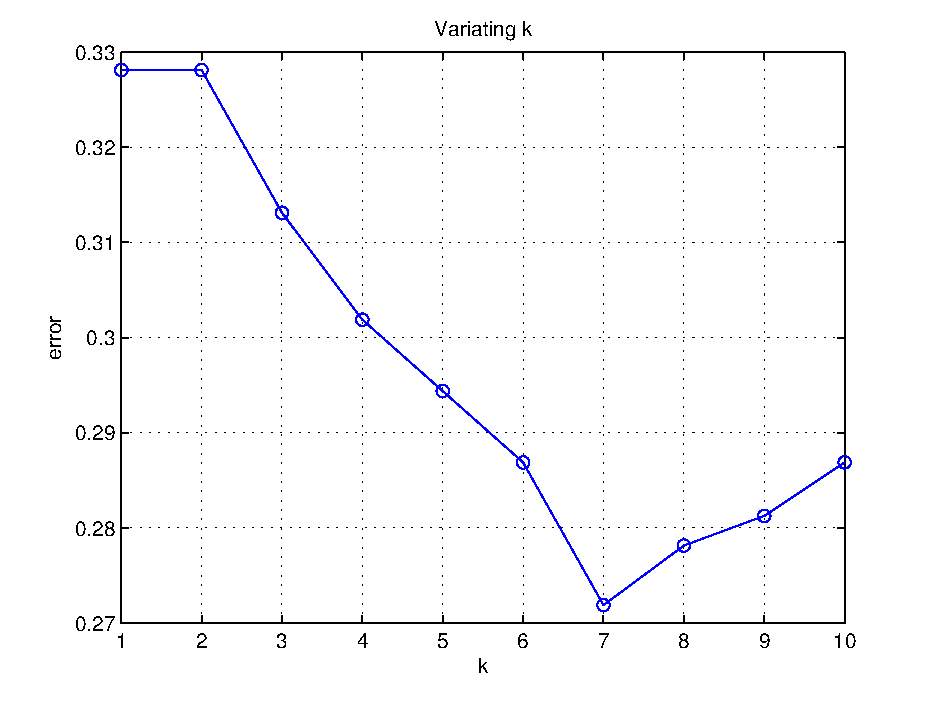
\includegraphics[width=0.6\textwidth]{./images/q207_best_k.pdf}
  \caption{Test error for variating N with 200 training points.}
  \label{fig:q27.1}
\end{figure}

Figure \ref{fig:q27.2} shows the optimal values of $k$ for different
number of points $N$ in the training set.  Seemingly, as $N$ grows,
$k$ needs to be larger for the error to be minimized (apart from the
spike around $50-70$).  This seems reasonable, as the additional
training points will cause the model to be more prone to over-fitting.
When more training points are used, but $k$ is raised correspondingly,
the level of detail, and therefore the error, in the model will remain
optimal.

\begin{figure}[!htbp]
  \centering
  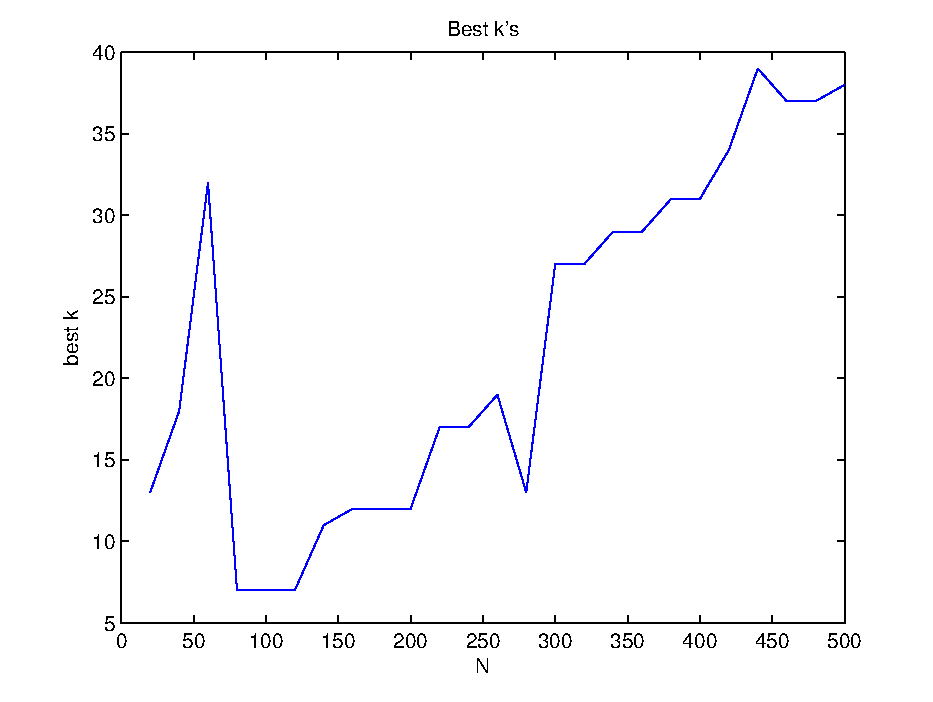
\includegraphics[width=0.6\textwidth]{./images/q207_best_ks.pdf}
  \caption{Best k's (lowest test error) for variating N.}
  \label{fig:q27.2}
\end{figure}
